\documentclass{report}
\usepackage{graphicx}
\usepackage{ragged2e}
\usepackage{amsmath}
\usepackage{listings}
\usepackage{color}

\definecolor{codegreen}{rgb}{0,0.6,0}
\definecolor{codegray}{rgb}{0.5,0.5,0.5}
\definecolor{codepurple}{rgb}{0.58,0,0.82}
\definecolor{backcolour}{rgb}{0.95,0.95,0.92}

\lstdefinestyle{mystyle}{
	backgroundcolor=\color{backcolour},   
	commentstyle=\color{codegreen},
	keywordstyle=\color{magenta},
	numberstyle=\tiny\color{codegray},
	stringstyle=\color{codepurple},
	basicstyle=\footnotesize,
	breakatwhitespace=false,         
	breaklines=true,                 
	captionpos=b,                    
	keepspaces=true,                 
	numbers=left,                    
	numbersep=5pt,                  
	showspaces=false,                
	showstringspaces=false,
	showtabs=false,                  
	tabsize=2
}

\lstset{style=mystyle}
\usepackage[british]{babel}
\usepackage[backend=biber, style=numeric, sorting=none]{biblatex}
\graphicspath{{img/}}
\usepackage[perpage]{footmisc}
\addbibresource{bib/database.bib}
\DefineBibliographyStrings{english}{%
	bibliography = {References},
} 
\usepackage{varwidth}
\usepackage{csquotes}
\usepackage{float}
\usepackage{algorithm}
\usepackage{algpseudocode}
\usepackage{listings}
\usepackage{tikz}
\usetikzlibrary{shapes, arrows}
\newcommand{\insertimage}[2] {
	\begin{figure}[H]
		\centering
		\includegraphics[width=\textwidth,height=\textheight,keepaspectratio]{#1}
		\caption{#2}
\end{figure}}
\begin{document}
\centering

\includegraphics[width=0.15\textwidth]{New_King_Edward_VI_Logo}\par\vspace{1cm}
{\scshape\LARGE King Edward VI Southampton\par}
\vspace{1cm}
{\scshape\Large A Level Coursework\par}
\vspace{1.5cm}
{\huge\bfseries Physics Revision Program\par}
\vspace{2cm}
{\Large\itshape Tom Eaton\par}
\vfill
supervised by\par
Mr. \textsc{Allen} and Mr. \textsc{Mapstone}

\vfill
{\large \today\par}

\tableofcontents
\begingroup
\let\clearpage\relax
\listoffigures
\listofalgorithms
\endgroup
\justifying
\chapter{Analysis}
\section{Abstract}
As I am an A Level Maths (with mechanics) and Physics student, I have studied the topics of projectile motion and radioactive decay. I myself found these topics to be difficult as did many other of my peers. The current method of practising mathematics and physics questions is to attempt problems from a course textbook. As there are many questions for the student to try, they can seem repetitive or boring causing the student to be more likely to stop. This can be solved by providing a range of questions to provide variety. The majority of problems are provided with no diagram, so the student has to interpret the text and potentially draw their own diagram. While this type of question is likely to come up in the exam, when the student is first learning the topic, it is important that they understand the topic fully before attempting harder, exam style questions. This can be solved by providing diagrams for the student. This allows the question text to be represented visually which make the problem easier to understand, and it will allow the student to relate the question to the underlying concepts that they are learning.

This software will be an easy to use platform. It will generate questions from the projectile motion and radioactive decay topics, and will draw graphs to go with these. The main aim of the software is to be a learning tool, to help students understand the basics of these topics.
\section{Features of the proposed solution that can be solved using computational methods}
\subsection{Random nature of questions}
The questions will be randomly generated. The base question will be stored so that there are elements within it that can be changed. This allows a loop to be created, which will produce \textit{n} amount of questions, with the elements being changed to a random number from a specified range. The generated elements can then be used to create the diagram or graph, by putting these elements into the diagram generation function.
\subsection{Answer Verification}
The number of significant figures in the student will not matter. If the student's answer is the same as the calculated answer to any number of significant figures it will be marked as correct. Computationally, this can be implemented by using built in \textbf{round} functions, meaning that the mathematics behind this does not have to be coded from scratch. This will be faster than if this was implemented non-computationally.
\subsection{Generation of diagrams}
For both projectile motion and radioactive decay, graphs can be generated using an iterative method. This works by supplying an equation with a variable that can be incremented. This is usually time \textit{t}. The equation then outputs a value that plotted as the y coordinate on a graph, with the x coordinate being the time value inputted into the equation. This solution will enable graphs of projectile motion and radioactive decay to be quickly generated for display.
\section{Stakeholders}
Students studying A Level physics are the main target users of this program. It will offer an unlimited supply of questions to practice outside of the textbook. The questions will be provided with a graph or diagram which could make the question seem easier to some. This is intended, as the program is meant to aid understanding of the fundamentals of these topics. 
A Level physics teachers are another target group. They will be able to use this tool in initial lessons to demonstrate how to answer these type of questions. The generated graph will enable easy explanation of the question, and will save time for the teacher. Once the basics have been covered, teachers could task students to complete questions on the application.
\clearpage
\section{Existing Solutions}
\begin{figure}[h]
	\centering
	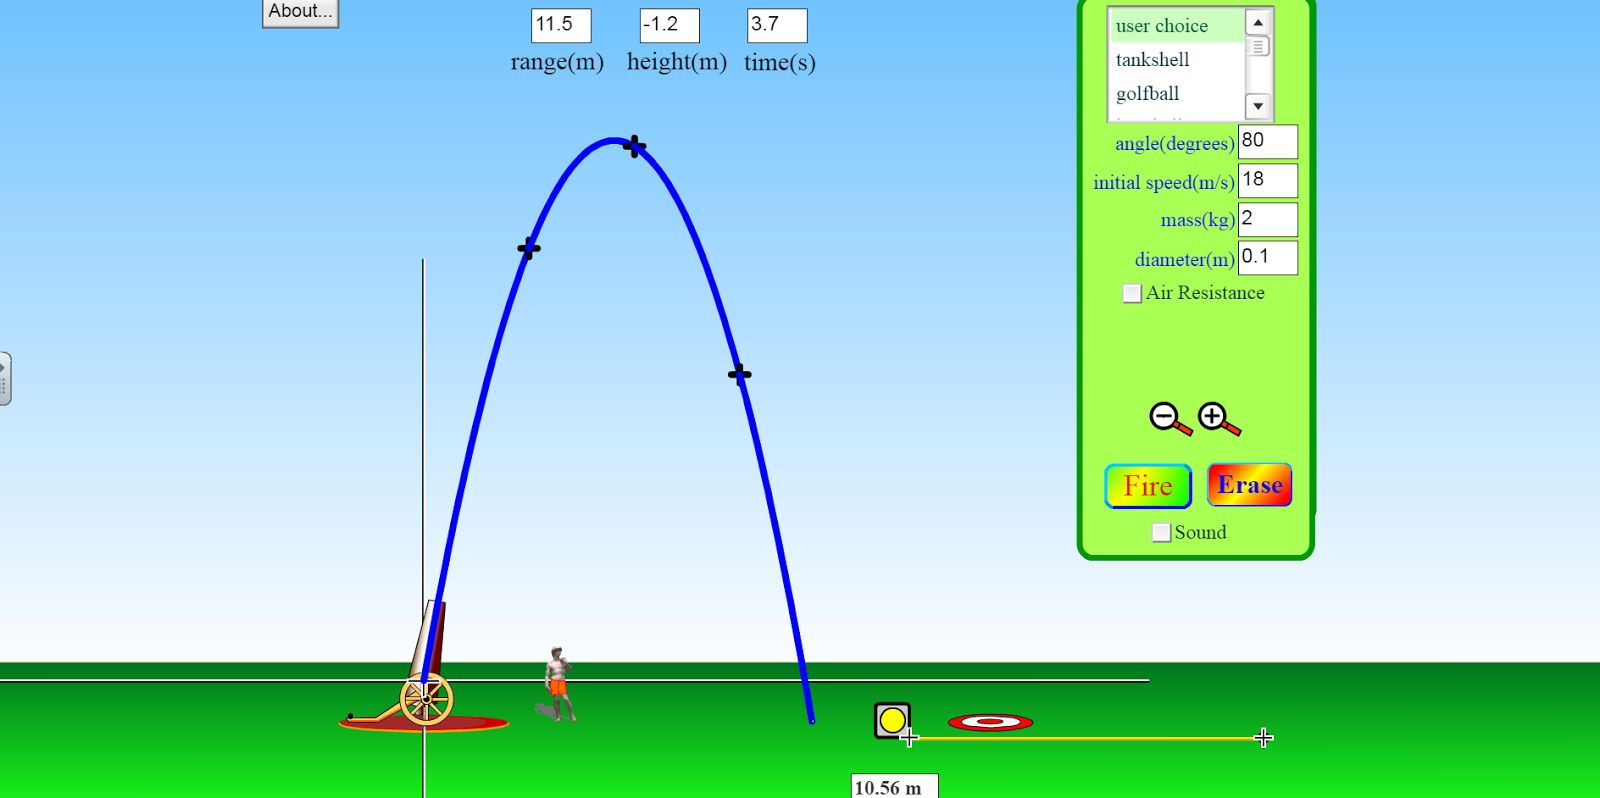
\includegraphics[width=\textwidth,height=\textheight,keepaspectratio]{Analysis-000}
	\caption[PHET Interactive projectile motion simulator.]{PHET Interactive projectile motion simulator. \autocite{phet}}
	\label{phet}
\end{figure}
This piece of software display the path of an object fired out of a cannon. You can modify the mass and diameter of the object being fired. This will only change the motion of the object if air resistance is being simulated. This simulation does have an option to enable air resistance, which will provide a more realistic simulation. However air resistance is not taken into account in the A Level Physics exam, so this feature will be left out. The launch speed and angle can also be changed. The graph generation should have changeable parameters, so that the values in the question can be used to produce a graph of itself. The user won't be allowed to directly change these values, as this is a question generation program, not a sandbox.
\clearpage
\begin{figure}[h]
	\centering
	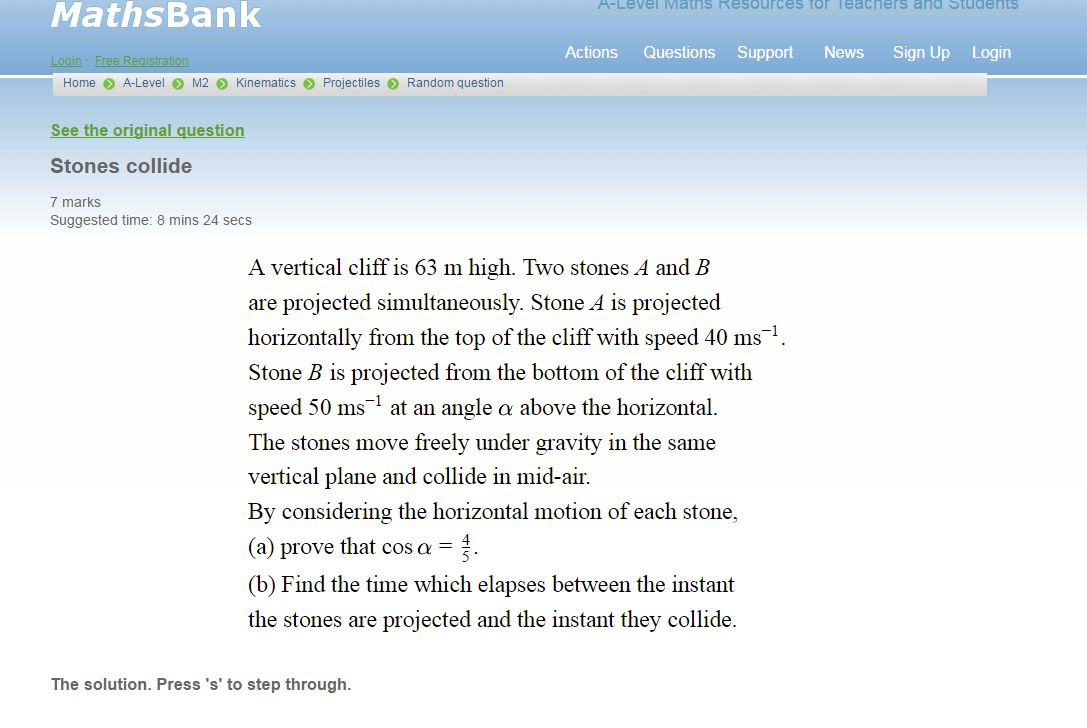
\includegraphics[width=\textwidth,height=\textheight,keepaspectratio]{Analysis-001}
	\caption[MathsBank M2 Projectile motion question bank.]{MathsBank M2 Projectile motion question bank. \autocite{mb}}
\end{figure}
This is an example of an exam style question. The question provides good context, making it easy to understand. A diagram is not provided, as it is expected that the student draws one for themselves. This type of question is not aimed at people just starting the topic, so the style of the question would have to be changed so that all of the information required is displayed obviously, rather than it being hidden in the text.
\clearpage
\begin{figure}[h]
	\centering
	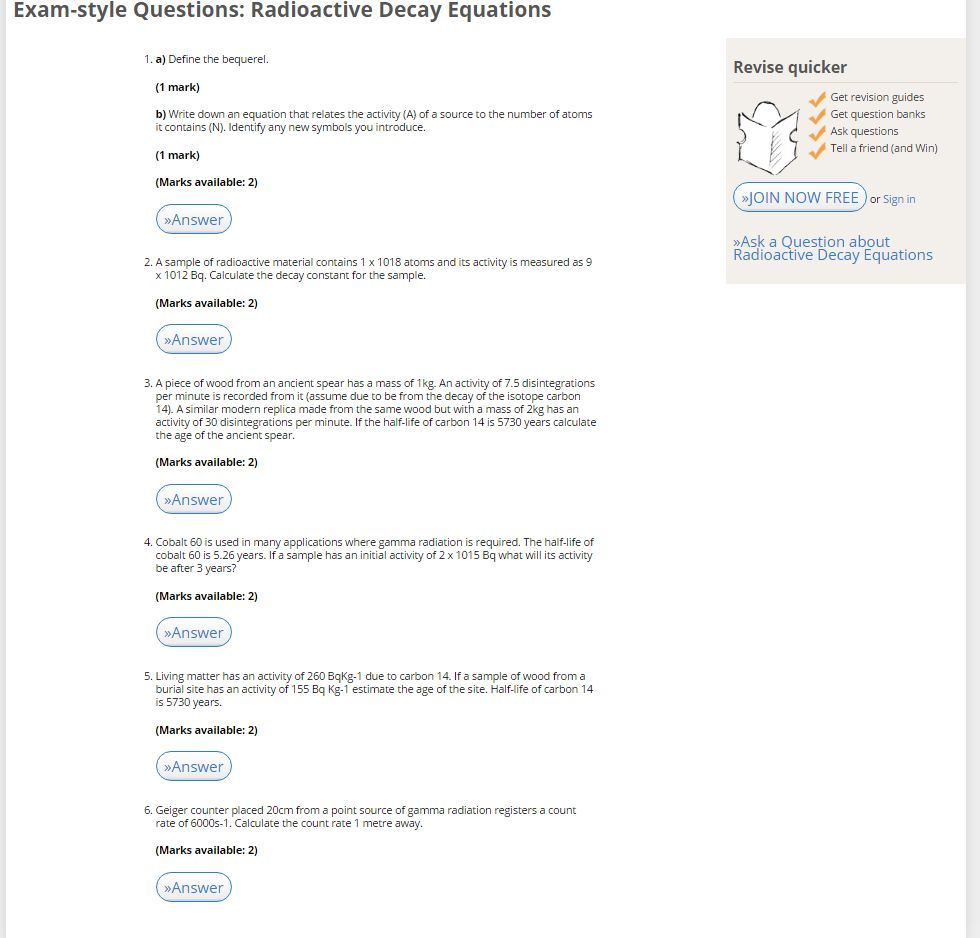
\includegraphics[width=\textwidth,height=\textheight,keepaspectratio]{Analysis-002}
	\caption[Exam-style Questions: Radioactive Decay Equations.]{Exam-style Questions: Radioactive Decay Equations. \autocite{scool}}
\end{figure}
These questions are extensive, and with a realistic context, making it more approachable to the student. Some of the questions are not suitable for random variation like Question 1, which are purely fact recall questions. The style of the other questions are ideal, as they are not too complex, and allow a graph or diagram to be drawn based off the information in the question.
\section{Solution}
\subsection{Question generation}
\subsubsection{Projectile motion}
The structure of the questions generated will be based on the MathsBank\autocite{mb} questions. The length of the question will be much shorter, only containing one part. This will avoid boredom from similar questions, and will avoid problems with the student having to remember answers to previous parts in order to correctly solve the next part. 
\begin{figure}
	\centering
	A ball is projected with speed \(x \text{ ms}^{-1}
	\). At the starting point the ball is \(S\) m of the ground. The highest point of the ball is \(y\)  m.
	\caption{Example projectile motion question.}
	\label{expm}
\end{figure}
\ref{expm} shows an example question, which is the style that will be generated for the user. The parameters which will be changed \(x, S \text{ and } y\) are obvious to the user, and no extra calculations are required. All of the information required to answer the question is easily shown in the question.
\subsubsection{Radioactive Decay}
The questions used in the program will be very similar to the questions found on S-cool\autocite{scool}. The only changes will be that the fact recall questions will be removed, due to that fact that these can't be truly randomised.
\begin{figure}[h]
	\centering
	A sample of radioactive material contains \(n\) atoms and its activity is measured as \(x\) Bq. Calculate the decay constant for the sample.
	\caption{Example radioactive decay question.}
	\label{exrd}
\end{figure}

Again, this shows how easy it is to randomise the question, with only the letter variables in \ref{exrd} having to be changed.

\subsection{GUI}
The GUI for the two different topics will be very similar, as they both have three distinct elements:	
\begin{itemize}
	\item{Question box}
	\item{Graph or diagram}
	\item{Answer box} 
\end{itemize}
The graph or diagram generated will be based on \ref{phet}, but it will be a much simpler version of this. Only two colours will be used, which will reduce confusion, and avoid distraction. There will also be no representation of the object being fired for clarity.
\section{Essential Features}
\begin{itemize}
	\item{Function GUI Menu.}
	\item{Clear distinction between two topics to avoid confusion.}
	\item{Questions with random variables.}
	\item{Simple random variables that are realistic for the question type.}
	\item{Verification of student's answer. Answer is accepted to any amount of significant figures.}
	\item{Graph or diagram to supplement question.}
\end{itemize}
\section{Limits of proposed solution}
The main issue with this solution is that the questions won't be truly random. This is because only parts of the question are randomised. For example looking at \ref{expm} and \ref{exrd} only the letter variables are randomised. There will be a small number of base questions, which determine the style of question and this cannot be randomised as it is out of the scope of this project. For the target user of this program, this won't be a problem. They won't be using the program for too long, as they will learn the basics and then move on to harder questions. In the time that it takes to do that, they won't have time to just learn how to answer the specific type of question, instead of learning the theory behind the question.

\section{Project Requirements}
\subsection{Programming language}
Python 3.5 will be the main project requirement as it is the programming language that the software will be written in. This language is being used because of the great number of libraries available to make the development process easier, and because it is portable, so can run on any modern computer.
\subsection{GUI}
To create the GUI, PyQt will be used, which is a python wrapper for QT. Qt is a cross-platform application framework that is used for developing application software that can be run on various software and hardware platforms with little or no change in the underlying codebase\autocite{qt}.This library will allow portability, and the code won't have to be rewritten due to it being a Python wrapper. Qt comes with a WYSIWYG\footnote{What you see is what you get.} editor called QtCreator, which is similar to the Visual Basic form designer. A GUI can be easily created using this, as it can be made visually, instead of having to make it in code, which is time consuming and can be hard to get right. Once the GUI is made in QtCreator, PyUIC5 can be run to convert the Qt code into Python code which can be used to display the GUI.
\subsection{Graph generation}
Matplotlib\footnote{Python Library used for plotting graphs.} will be used to generate the graph and diagram for display on the GUI. It is easy to use, and executes quickly, which is important to reduce waiting time for the user. The matplotlib window will not be shown directly to the user, matplotlib will be called to generate an image of the graph which will then be displayed. This is to make sure that there is no issues with graph size.
\subsection{Hardware requirements}
The only requirement is a relatively modern PC, that is running a contemporary operating system. 
\subsection{Final Build}
The final build of the software will have a .exe file that will be run by the user. The Python libraries still need to be available to the program, so they need installed on the computer. This can be done in two ways, either by installing the Anaconda Python distribution, or providing a virtualenv\footnote{An isolated Python environment} with the libraries installed. A virtualenv would be easier for the user, as they don't have to install any additional software.
\section{Success Criteria}
\begin{itemize}
	\item Functional, easy to use GUI.
	\item Randomly generated questions
	\item Realistic values in question
	\item Random question is shown to the user within a second of page display
	\item Graph or diagram generated in relation to question
	\item Graph is displayed within a second
	\item Student's answers are verified and correct no matter the amount of significant figures.
\end{itemize}
\tikzstyle{datastore} = [rectangle, draw=black, fill=white, text width=5em, text centered, rounded corners, minimum height=4em]
\tikzstyle{system} = [ellipse, draw=black, fill=white, text centered, minimum height =10em, minimum width=15em]
\tikzstyle{process} = [rectangle, draw=black, minimum width=8em, minimum height= 7em, text centered]
\tikzstyle{entity} = [rectangle, draw=black, minimum width=5em, minimum height= 4em, text centered]
\tikzstyle{processtop} = [rectangle, draw=black, minimum width=8em, minimum height=2em, text centered]
\tikzstyle{datastore} = [rectangle, draw=black, minimum width=12em, minimum height=2em, text centered]
\tikzstyle{datastorebox} = [rectangle, draw=black, minimum width=2em, minimum height=2em, text centered]
\chapter{Design}
\section{Design Overview}
The whole project can be broken down into three parts
\begin{itemize}
	\item Generation of question.
	\item Generation of graph / diagram.
	\item Display of GUI.
\end{itemize}
\subsection{Generation of question}
To be able to generate the questions randomly on the fly, a bare question structure must be implemented. To create this question structure, questions found in Figure \ref{fig:mb} for example, are analysed to find the variables that are important to the question. These are highlighted in Figure \ref{expm} as the lettered variables. Once these variables are found, the question is written in a text file in a way that the variables can be formatted to what is required.
\subsection{Generation of graph / diagram} 
Matplotlib will be used to generate the graph as discussed earlier. It will require an equation to be able to do this. The equation could be stored in the question in the text file, but it would be easier to just store the question type in the text file. You could then code specific equations depending on the question type. This will prevent the text file from getting too long and hard to read. It will also improve runtime performance, as it will be a shorter and less complex string to parse. The graph will be generated as an image.
\subsection{Display of GUI}
The display of the GUI will take the generated question, and the image of the graph and collate them to show the GUI. Apart from this, the GUI needs to be able to take a user answer, and check if it is correct. It will need to provide buttons to select a topic, submit an answer and skip a question.
\section{Dataflow diagrams}
\begin{figure}[H]
\centering
\begin{tikzpicture}[node distance = 2cm]
	\node [system] (system)at (0, 0) {System};
	\node [entity, right of=system, xshift=10em] (student) {Student};
	\draw [->, transform canvas={yshift=1em}] (student) -- node[anchor=south] {Answer} (system) [yshift=1em];
	\draw [<-, transform canvas={yshift=-1em}] (student.west) -- node[anchor=south] {Question} (system) [yshift=1em];
\end{tikzpicture}
\caption{Level 0 Dataflow Diagram}
\end{figure}
\begin{figure}[H]
\centering
\begin{tikzpicture}
	\node [entity] (student1) {Student};
	\node [process, right of=student1, xshift=8em, label={[yshift=-5em]Load Question}] (ldquestion) {};
	\node [processtop, above of=ldquestion, yshift=-.35em] (ldquestiontop) {1};
	\draw [->] (student1) -- node[anchor=south] {Topic} (ldquestion);
	\node [process, right of=ldquestion, xshift=12em, text width=3em, label={[yshift=-6.25em]\begin{varwidth}{5em}Generate random variables\end{varwidth}}] (randomgen) {};
	\node [processtop, above of=randomgen, yshift=-.35em] (randomgentop) {2};
	\draw [->] (ldquestion) -- node[anchor=south, yshift=.1em] {Generation} node[anchor=north, yshift=-.1em] {range} (randomgen);
	\node [datastore, below of=randomgen, yshift=-8em, label={[yshift=-1.85em, xshift=1em]\small Temporary variables}] (tempvar) {};
	\node [datastorebox, left of=tempvar, xshift=-2.15em] (tempvarside) {D1};
	\draw [->] (randomgen) -- node[anchor=west] {\begin{varwidth}{5em}Random variables\end{varwidth}}(tempvar);
	\node [process, left of=tempvar, xshift=-11em, text width=3em, label={[yshift=-5.8em]\begin{varwidth}{5em}Format question\end{varwidth}}] (questionformat) {};
	\node [processtop, above of=questionformat, yshift=-.35em] (questionformattop) {3};
	\draw [->] (tempvar) -- node[anchor=south] {\small Random} node[anchor=north]{\small variables}(questionformat);
	\node [entity, below of=questionformat, yshift=-6em] (student2) {Student};
	\draw [->] (questionformat) -- node[anchor=west] {Question} (student2);
	\node [process, left of=questionformat, xshift=-9em, text width=3em, label={[yshift=-5.8em]\begin{varwidth}{5em}Validate answer\end{varwidth}}] (answervalidate) {};
	\node [processtop, above of=answervalidate, yshift=-.35em] (questionformattop) {4};
	\draw [->] (questionformat) -- node[anchor=south] {\small Answer}(answervalidate);
	\draw [->] (student1) -- node[anchor=west] {\begin{varwidth}{3em}Student answer\end{varwidth}}(answervalidate);
	\draw [->] (answervalidate) |-  node[anchor=south, yshift=-2em, xshift=4.5em] {Feedback}(student2) ;
	\draw [->] (ldquestion) -- node[anchor=west] {Empty question}(questionformat);
\end{tikzpicture}
\caption{Level 1 Dataflow Diagram}
\label{dfd}
\end{figure}
Figure \ref{dfd} shows the main flow of the program. As you can see, most of the code will be written to perform the generation of the question, as this is the most complex part.

\section{Algorithms}
N.B In all of these algorithms the classes defined in Section 2.5 will be referenced.
\begin{algorithm}
	\label{mainps}
	\caption{Main Algorithm}
	\begin{algorithmic}[1]
		\State Display MainMenu
		\If {Projectile topic button pressed}
			\State new ProjectileQuestion
			\State loadQuestion from projectile.txt
			\State ProjectileQuestion(loadQuestion)
			\If{RadioactiveQuestion.answer = student answer}
			\State print "You got it right"
			\State ProjectileQuestion(loadQuestion)
			\Else
			\State print "You got it wrong"
			\State ask "Would you like to see the answer"
			\If {yes}
			\State print ProjectileQuestion.answer
			\State RadioactiveQuestion(loadQuestion)
			\Else
			\State return to function
			\EndIf
			\EndIf
		\EndIf
		\If {Radioactive decay pressed}
			\State Display RadioactiveQuestion
			\State loadQuestion from radioactive.txt
			\State RadioactiveQuestion(loadQuestion)
		\EndIf
		\If {Close button pressed}
			\State Display PromptBox("Are you sure about that"?)
			\If{Answer = True}
				\State Close application
			
			\Else
				\State Go to MainMenu
			\EndIf
		\EndIf
	\end{algorithmic}
\end{algorithm}
\subsection{Justification}
This is a simple overview of how the program will run. The only point of interest in this is the fact that when a user gets the question wrong, they are asked whether they would like to see the answer or try again. This was used to prevent infuriation if the student cannot get the answer, but to also allow students to try again if they think they are close to the answer. 

The main algorithm forms a complete solution as it covers all of the input that the user could give, for example wanting to retry the question or to see the answer.
\subsubsection{Algorithm run order}
The order that this algorithm will run will depend on the run time of each algorithm. For example, the diagram generation may take a long time to execute, so it may be beneficial to generate questions in advance, so that the user does not have to wait a long time when switching question. 

Ignoring this, the run order will be this:
\begin{enumerate}
	\item Let the user choose the topic.
	\item Generate the question and graph for that topic.
	\item Get the student's answer and check against real answer.
	\item If correct go back to step 2
	\item If incorrect ask user if they want to skip question or try again.
\end{enumerate} 


\section{Usability Features}
Usability features are an important part of this programs success. As the tasks that this program does could be done elsewhere, albeit at the cost of more effort, it is important that the program is as easy to use a possible. This can be resolved by adding key usability features.

The main usability feature is the easy to use GUI. It only has the essential functions, which may mean a small reduction in productivity. However, the GUI will be much more intuitive, and will lead to a more simple experience overall. This is crucial, as ease of use is the main reason that this is a problem.

The feedback on student's answers is another usability feature. If the student gets the answer wrong, they have the choice to either try again, or to see the answer and move onto the next question. The program could just not let you move on if you don't get the right answer, but this could lead to annoyance if they are stuck on a question.

\section{Datastructures}
\subsection{Classes}
\algrenewcommand\algorithmicprocedure{\textbf{Class}}
\algblock[public]{public}{endpublic}
\algblock[private]{private}{endprivate}
\begin{algorithm}[H]\label{randomised}
	\caption{Randomised}
	\begin{algorithmic}[1]
		\Procedure{Randomised}{}
		\public
		\State \textbf{Function} format
		\State \textbf{Function} get\_class
		\State \textbf{Function} get\_item
		\State \textbf{Function} get\_question\_class 
		\endpublic
		\private
		\State Question\_class : Class
		\endprivate
		\EndProcedure
	\end{algorithmic}
\end{algorithm}
\begin{algorithm}[H]\label{randomisedps}
	\caption{Randomised Pseudocode}
	\begin{algorithmic}[1]
		\Procedure{Randomised}{}
		\Function {init} {self}
		\State self.args $\gets$ []
		\State self.question $\gets$ None
		\EndFunction
		\Function {format} {string}
		\State formatter $\gets$ new RandomisedFormatter
		\State formatter.format(this object, string)
		\EndFunction
		\Function {getItem}{self, name}
		\State return RandomizedFormatter(name, self.args)
		\EndFunction
		\Function {getClass}{self}
		\If {self.args['equation'] = 'findtheta'}
		\State self.question $\gets$ ProjectileQuestion(self.args['a'], self.args['b'], self.args['c]))
		\EndIf
		\If {self.args['equation'] = 'findmaxheight'}
		\State self.question $\gets$ ProjectileQuestion(self.args['a'], self.args['b'], self.args['c']))
		\EndIf
		\If {self.args['equation'] = 'findxdistance'}
		\State self.question $\gets$ ProjectileQuestion(self.args['a'], self.args['b'], self.args['c]))
		\EndIf
		\If {self.args['equation'] = 'findradioactive'}
		\State self.question $\gets$ RadioactiveQuestion(self.args['a'], self.args['b'], self.args['c]))
		\EndIf
		\If {self.args['equation'] = 'findDecayConstant'}
		\State self.question $\gets$ RadioactiveQuestion(self.args['a'], self.args['b'], self.args['c]))
		\EndIf
		\If {self.args['equation'] = 'findParticles'}
		\State self.question $\gets$ RadioactiveQuestion(self.args['a'], self.args['b'], self.args['c]))
		\EndIf
		\EndFunction
		\EndProcedure
	\end{algorithmic}
\end{algorithm}
\begin{algorithm}[H]\label{randomisedFormatter}
	\caption{RandomisedFormatter}
	\begin{algorithmic}[1]
		\Procedure{RandomisedFormatter}{}
		\public
		\State \textbf{Function} format
		\State \textbf{Function} get\_name
		\State \textbf{Function} get\_args
		\endpublic
		\private
		\State name : String
		\State args : String Array
		\endprivate
		\EndProcedure
	\end{algorithmic}
\end{algorithm}
\begin{algorithm}[H]
	\label{randomformatterps}
	\caption{RandomisedFormatter Pseudocode}
	\begin{algorithmic}[1]
		\Procedure{RandomisedFormatter}{}
		\Function {init} {self, name, args}
		\State self.name $\gets$ name
		\State self.args $\gets$ args
		\EndFunction
		\Function {format} {self, fmt}
		\State op, rest $\gets$ fmt.split(':') \Comment text before ':' into op, text after into  rest
		\If {op == 'type'}
		\State self.args[self.name] = rest
		\State return None
		\EndIf
		\If {op == 'random'}
		\State low, high = rest.split(':')
		\State value $\gets$ randomNumber(low, high)
		\State self.args[self.name] $\gets$ value
		\State return string(value)
		\EndIf
		\EndFunction
		\EndProcedure
	\end{algorithmic}
\end{algorithm}
\begin{algorithm}[H]\label{ProjectileQuestion}
	\caption{ProjectileQuestion}
	\begin{algorithmic}[1]
		\Procedure{ProjectileQuestion}{}
		\public
		\State \textbf{Function} calculateProjectile
		\State \textbf{Function} findTheta
		\State \textbf{Function} findXdistance
		\State \textbf{Function} findMaxHeight
		\State \textbf{Function} calculatePoint
		\State \textbf{Function} getTheta
		\State \textbf{Function} getXdistance
		\State \textbf{Function} getMaxHeight
		\endpublic
		\private
		\State theta : Integer
		\State xdistance : Float
		\State maxHeight : Float
		\endprivate
		\EndProcedure
	\end{algorithmic}
\end{algorithm}
\begin{algorithm}[H]
	\label{projectilequestionps}
	\caption{ProjectileQuestion Pseudocode}
	\begin{algorithmic}[1]
		\Procedure{ProjectileQuestion} {}
		\Function {init}{self, yOffset, initialSpeed, theta}
		\State self.yOffset $\gets$ yOffset
		\State self.initalSpeed $\gets$ initialSpeed
		\State self.theta $\gets$ theta
		\EndFunction
		\Function {calculateProjectile}{}
		\State increment $\gets$ 0.01
		\State theta $\gets$ radians(theta)
		\State xSpeed $\gets$ self.initialSpeed * cos(theta)
		\State ySpeed $\gets$ self.initialSpeed * sin(theta)
		\State time $\gets$ 0
		\State time $\gets$ time + increment
		\State self.xPosArray $\gets$ []
		\State self.yPosArray $\gets$ []
		\State yPosTemp $\gets$ 5 \Comment To satisfy \texttt{while} loop during first run
		\While {yPosTemp > 0}
		\State xPosTemp $\gets$ xSpeed $\times$ time
		\State yPosTemp $\gets$ (ySpeed $\times$ time) + (0.5 * -9.8 * $\textrm{time}^2$ + self.yOffset) 
		\State xPosArray.append(xPosTemp)
		\State yPosArray.append(yPosTemp)
		\State time $\gets$ time + increment
		\EndWhile
		\EndFunction
		\Function {findTheta}{}
		\State self.calculateProjectile()
		\State plotAsImg(thetaDiagram, self.xPosArray, self.yPosArray, graph.png)
		\State resize(graph.png, 0.5)
		\State save(graph.png)
		\EndFunction
		\Function {findXDistance}{}
		\State self.calculateProjectile()
		\State plotAsImg(xDistanceDiagram, self.xPosArray, self.yPosArray, graph.png)
		\State resize(graph.png, 0.5)
		\State save(graph.png)
		\EndFunction
		\Function {findMaxHeight}{}
		\State self.calculateProjectile()
		\State plotAsImg(maxHeightDiagram, self.xPosArray, self.yPosArray, graph.png)
		\State resize(graph.png, 0.5)
		\State save(graph.png)
		\EndFunction
		\algstore{pqps}
		
	\end{algorithmic}
\end{algorithm}
\clearpage
\begin{algorithm}[H]
	\caption{ProjectileQuestion Pseudocode continued}
	\begin{algorithmic}[1]
		\algrestore{pqps}
		\Function {calculatePoint}{startX, startY, angle, length}
		\State endpoint $\gets$ [startX + (length $\times$ cos(angle)), startY + (length $\times$ sin(angle))]
		\State return endpoint
		\EndFunction
		\Function {answerTheta}{}
		\State return self.theta
		\EndFunction 
		\Function {answerXDistance}{}
		\State return max(self.xPosArray)
		\EndFunction
		\Function {answerMaxHeight}{}
		\State return max(self.yPosArray)
		\EndFunction
		\EndProcedure
	\end{algorithmic}
\end{algorithm}
\begin{algorithm}[H]\label{RadioactiveQuestion}
	\caption{RadioactiveQuestion}
	\begin{algorithmic}[1]
		\Procedure{RadioactiveQuestion}{}
		\public
		\State \textbf{Function} calculateDecay
		\State \textbf{Function} findDecayConstant
		\State \textbf{Function} findHalfLife
		\State \textbf{Function} findActivity
		\State \textbf{Function} findParticles
		\State \textbf{Function} getDecayConstant
		\State \textbf{Function} getHalfLife
		\State \textbf{Function} getActivity
		\State \textbf{Function} getParticles
		\endpublic
		\private
		\State decayConstant : Float
		\State halfLife : Float
		\State activity : Integer
		\State particles : Integer
		\endprivate
		\EndProcedure
	\end{algorithmic}
\end{algorithm}
\clearpage
\subsection{Variables}
\begin{center}
	\begin{tabular}{|c|c|c|}
		\hline
		\multicolumn{3}{|c|}{\textbf{Variables}}\\
			\hline
			\textbf{Variable name} & \textbf{Variable type} & \textbf{Comments}\\
			\hline
			MainApp & Class & Instance of the main menu class \\
			\hline
			temporaryObject & Class & Question generation class
			 \\
			\hline
			answer & Integer / float & Answer to the question \\
			\hline
			studentAnswer & Integer / float & Students answer \\
			\hline
		\end{tabular}
	\end{center}
\subsection {Explanation}
Algorithm 1 is the class definition for the \texttt{Randomised} class. It is used to call the \texttt{RandomisedFormatter} class in order to format the question string, and also to return the class.

Algorithm 2 is the pseudocode for the \texttt{Randomised}Class. The main bulk of the code is taken up by the getClass Function. This is used to verify
\subsection{Justification}
In Algorithm \ref{ProjectileQuestion} and \ref{RadioactiveQuestion} you can see that the Function names are similar, with there being a find function and a get function for each variable. This is because the find function is used to generate the question and answer, and the get function is used to return the variable. The get function is needed to allow the question to be formatted with data required to answer it.

Classes \texttt{Randomised} and \texttt{RandomisedFormatter} found in Algorithms \ref{randomised} and \ref{randomisedFormatter} respectively, were created using classes as this was required to extend the inbuilt Python string formatter. By default, \texttt{str.format()} replaces fields delimited by braces\autocite{pystr}.
\begin{figure}[H]
	\centering
	\texttt{>>> "The sum of 1 + 2 is {0}".format(1+2)}\\
	\texttt{'The sum of 1 + 2 is 3'}
	\caption{Default behaviour of Python's \texttt{str.format()}\autocite{pystr}}
\end{figure}
The \texttt{RandomisedFormatter} Class extends this functionality, by allowing custom arguments to be specified in the brace delimiter, instead of just a keyword argument, or an index argument. 
\begin{figure}[H]
	\label{exformat}
	\centering
	\texttt{A ball is projected with speed \{a:random:20:40\}. At the starting point the ball is \{b:random:5:30\}m of the ground. The highest point of the ball is \{equation:type:findtheta\}}
	\caption{Example string for extended string formatter}
\end{figure}
The syntax in Figure \ref{exformat} allows an operand to be specified, and an operator. If necessary, further arguments provided for example a range of values. In the string argument \texttt{\{a:random:20:40\}} \texttt{a} is the operand, and this is the name of the variable in which the random number will be stored. \texttt{random} specifies the operation to be performed, in this case generate a random number. Finally \texttt{20:40} specifies the range for the random number generation.

The \texttt{\{equation:type:findtheta\}} is less complex, and just allows the equation type to be associated with the string, so the program knows what calculations to perform.

\subsubsection{Variables}
The variables shown in this section are the main variables that will be used. There are many other variables, but these are mostly covered in the class definitions so are not not worthy. The temporary object is probably the most important variable. This is because as the question generation is random, you need to keep track of the random variables so that you can get an answer from it. This solves the problem by allowing constant access to the class which was instantiated with the random variables, so that you can call methods on that class to get the answer and other things. The \texttt{studentAnswer} and \texttt{answer} are also important, so that the students answer can be verified.
\subsection{Validation}
The only variable that will require validation is \texttt{studentAnswer}. This is because it is user input. The variable will need to be checked that it only contains numbers only. Spaces won't have to be stripped from the variable, as this is automatically done by Python.
\section{Test data}
Test data will be important in determining the order in which the algorithms run, as it is critical that the questions don't take too long to display. The areas to be tested will be shown below.
\begin{itemize}
	\item Time to generate question
	\item Time to display graph/diagram
	\item Generation of variables within question are in specified range
	\item Graph has a reasonable scale so that the information is easy to read
	\item Graph image is high enough resolution to be seen clearly
\end{itemize}
The time to generate question and display graph are being tested so that changes to the algorithm order can be made if necessary. If it takes too long to generate the question, then this will no longer be done at runtime, so that the user doesn’t have to wait for the question to be generated. Checking that the variables are within a reasonable range is done so that the questions are realistic. For example it would not be realistic for a sample of material to have 12 atoms in it. Checking that the graph has reasonable axis is done so that the graph is easy to read, and fits well into the space. It would not be helpful if only a small part of the graph is being shown, and neither would it be helpful if too much of the graph was shown. The right amount of graph to show will be refined during user testing. Testing that the graph image is high enough resolution is done partly to make sure that the image can be seen clearly on the GUI, but it also links back to the time to display graph. If the image resolution is greater, then it will take longer to create, but will be easier to see. During testing I will have to find a balance point between resolution and time to create.

\chapter{Development}

\printbibliography[heading=bibintoc]
\end{document}